\documentclass[10pt,letterpaper]{article}

\usepackage[spanish,es-noquoting]{babel}
\usepackage[letterpaper,top=1.45cm,bottom=1.45cm,left=1.65cm,right=1.65cm]{geometry}
\usepackage{xcolor}
\usepackage{graphicx}
\usepackage{tabularx}
\usepackage{array}
\usepackage{enumitem}
\usepackage{microtype}
\usepackage[hidelinks]{hyperref}

\definecolor{SoftGray}{HTML}{F3F4F6}
\definecolor{RuleGray}{HTML}{D6DADF}
\definecolor{TextGray}{HTML}{444444}

\setlength{\parindent}{0pt}
\setlength{\parskip}{0.45em}
\setlength{\fboxsep}{7pt}
\setlist[itemize]{leftmargin=1.15em,itemsep=0.14em,topsep=0.15em}
\pagestyle{empty}
\raggedbottom

\newcommand{\sectiontitle}[1]{%
  \vspace{0.55em}%
  {\bfseries\large #1}\par
  \vspace{0.12em}%
}

\newcommand{\smallsection}[1]{%
  \vspace{0.35em}%
  {\bfseries #1}\par
}

\newcommand{\imagecaption}[1]{%
  \vspace{0.25em}{\footnotesize\color{TextGray}#1}\par
}

\newcommand{\infobox}[1]{%
  \noindent\colorbox{SoftGray}{%
    \begin{minipage}{0.965\textwidth}
    #1
    \end{minipage}}%
}

\begin{document}

{\LARGE\bfseries Aula Subtitulada AIEP}\par
{\normalsize Resumen breve para Dirección | Concurso Innovación Docente 2026}

\vspace{0.35em}
{\color{RuleGray}\rule{\textwidth}{0.6pt}}

\sectiontitle{Resumen ejecutivo}

\infobox{%
\textbf{Aula Subtitulada AIEP} es una aplicación de apoyo pedagógico que muestra subtítulos flotantes en tiempo real durante la clase. El docente usa su celular como micrófono; el computador recibe la transcripción y presenta el texto sobre la presentación, navegador, aula virtual o herramienta que esté usando.
}

\vspace{0.35em}
\begin{tabularx}{\textwidth}{>{\bfseries}p{4.25cm}X}
Foco principal & Accesibilidad e inclusión en aula, con tecnología como medio de apoyo. \\
Postulante y líder & Diego Matías Obando Aguilera. \\
Impulsor institucional & Elias Alberto Silva Carrasco, Jefe Escuela Ingeniería, Energía y Tecnología, sede Osorno. \\
Línea propuesta & Innovación en el Aula. \\
\end{tabularx}

\sectiontitle{Interfaz docente}

\begin{center}
\begin{minipage}[t]{0.485\textwidth}
  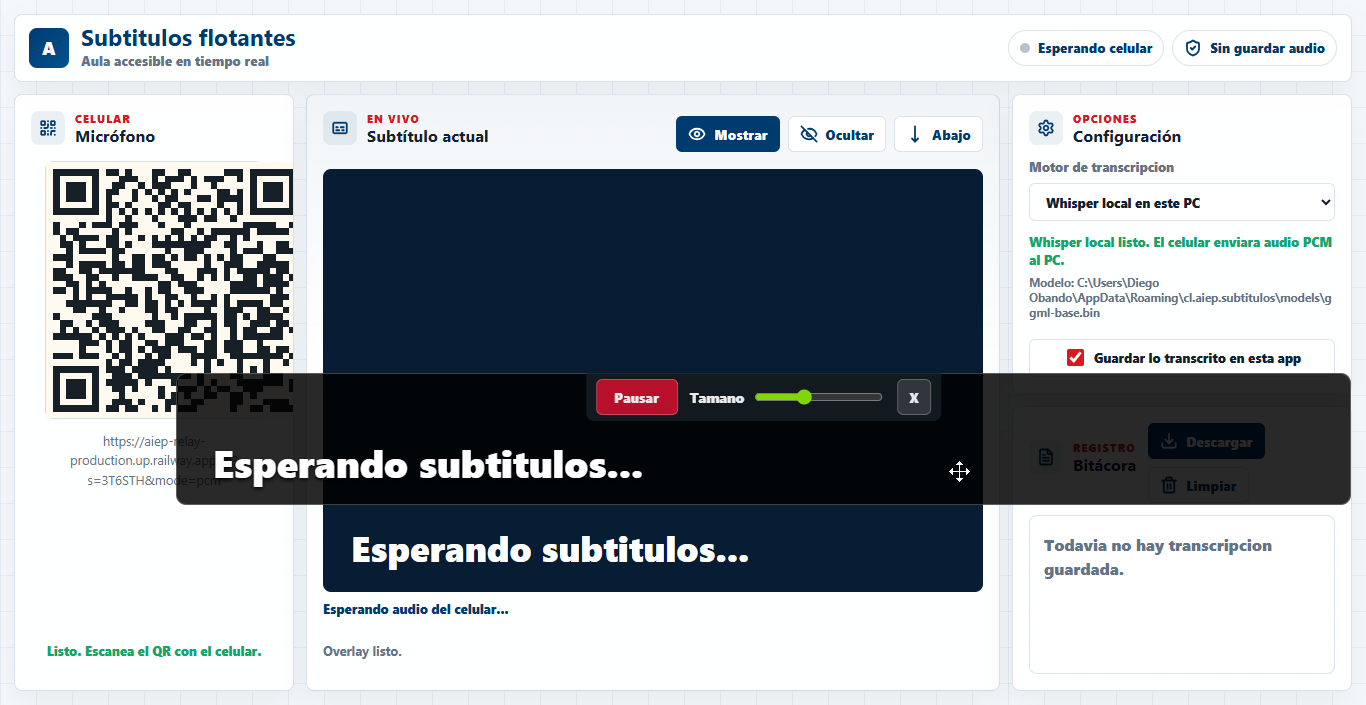
\includegraphics[width=\linewidth]{postulacion-assets/desktop-overlay-esperando.png}
  \imagecaption{\textbf{Vista general en PC.} La app muestra el QR, configuración y subtítulo flotante.}
\end{minipage}
\hfill
\begin{minipage}[t]{0.485\textwidth}
  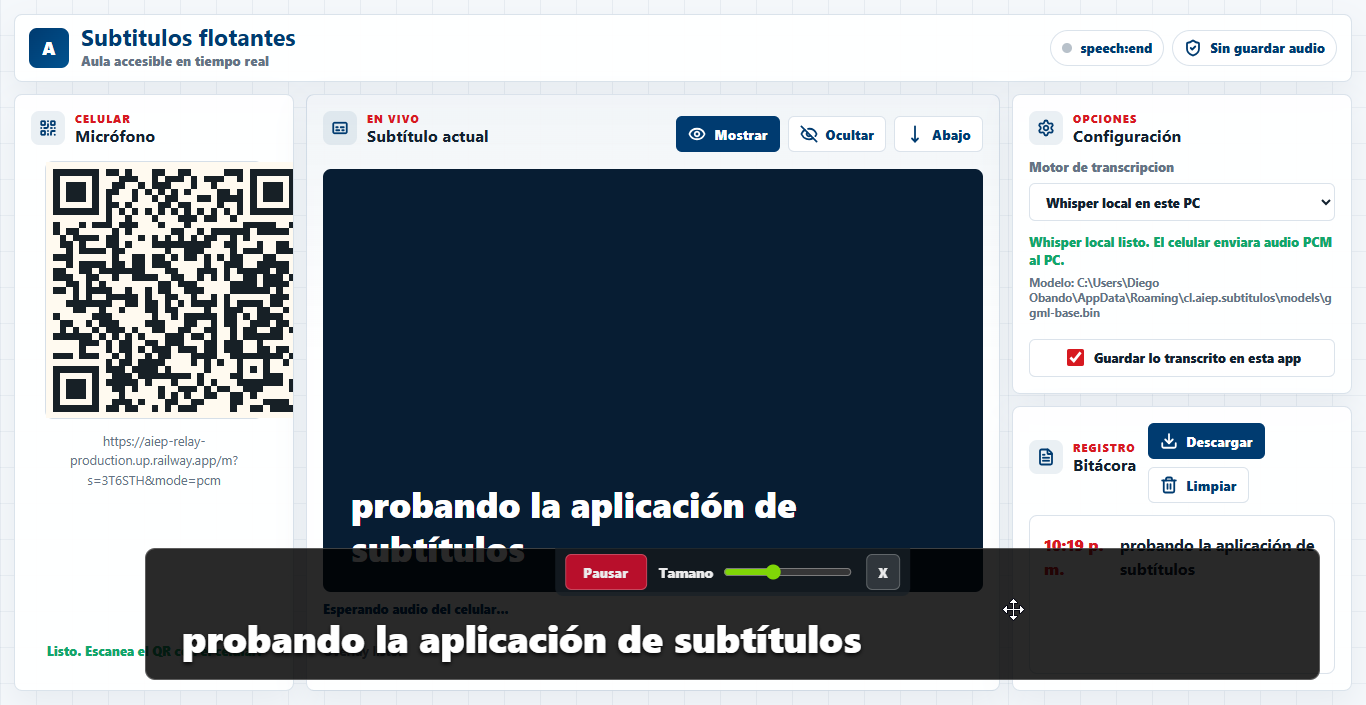
\includegraphics[width=\linewidth]{postulacion-assets/desktop-overlay-transcribiendo.png}
  \imagecaption{\textbf{Subtitulado activo.} Lo hablado se presenta como texto visible y movible.}
\end{minipage}
\end{center}

\sectiontitle{Uso en clase}

\begin{tabularx}{\textwidth}{>{\bfseries}p{0.8cm}X}
1 & El docente abre la aplicación en el computador. \\
2 & Escanea el QR con su celular y activa el micrófono. \\
3 & La voz se transforma en subtítulos visibles en tiempo real. \\
4 & Con autorización, la transcripción puede servir para generar resúmenes, glosarios, fichas o infografías. \\
\end{tabularx}

\smallsection{Aporte esperado}
\begin{itemize}
  \item Reduce barreras de acceso al discurso oral: audición, atención, lenguaje, ubicación en sala o vocabulario técnico.
  \item Se basa en Diseño Universal para el Aprendizaje: el apoyo queda disponible para todo el curso.
  \item Es replicable con recursos simples: computador docente, celular y guía de implementación.
\end{itemize}

\newpage

{\LARGE\bfseries Vista móvil y proyección pedagógica}\par
{\normalsize Aula Subtitulada AIEP | Resumen para Dirección}

\vspace{0.35em}
{\color{RuleGray}\rule{\textwidth}{0.6pt}}

\sectiontitle{Micrófono desde celular}

\begin{center}
\begin{minipage}[t]{0.34\textwidth}
  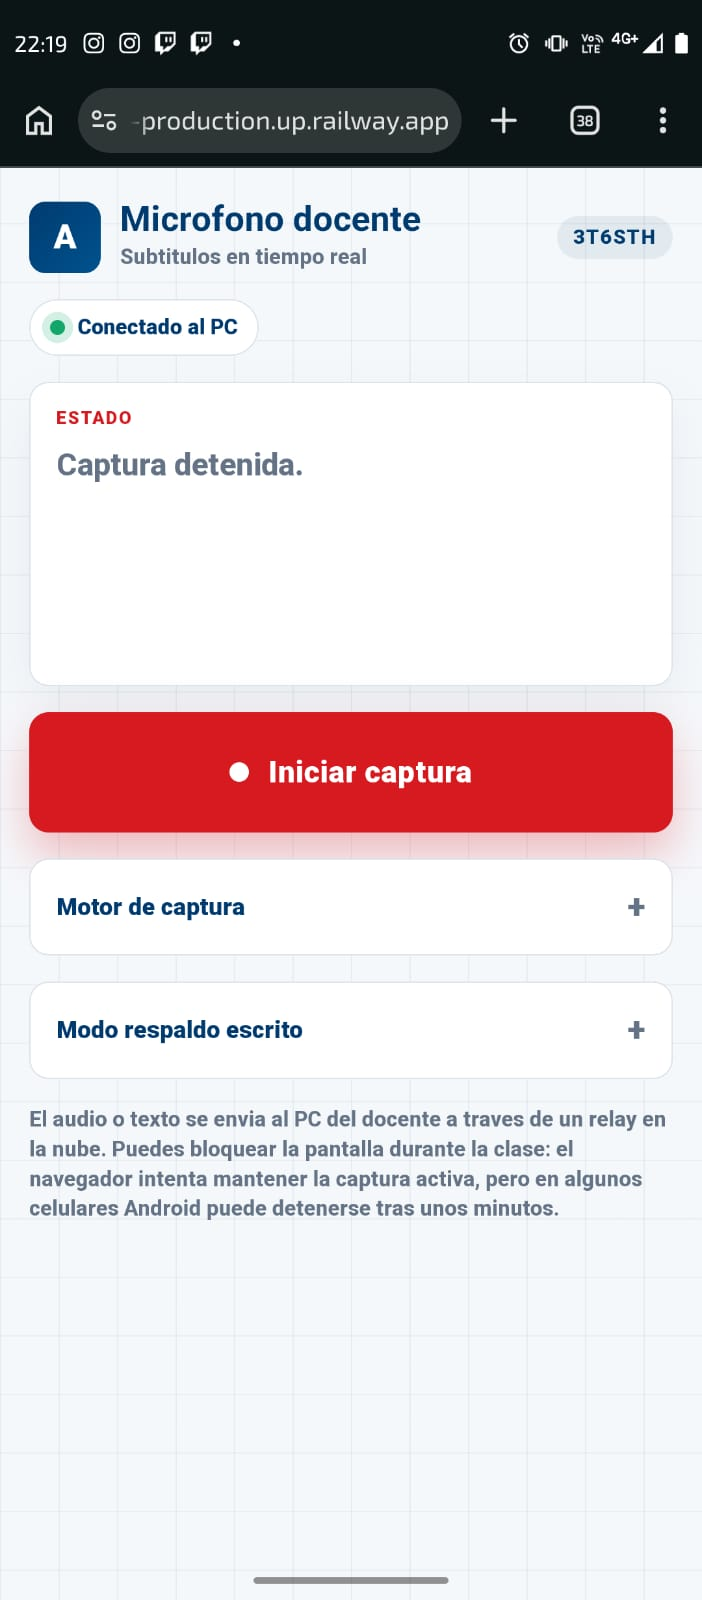
\includegraphics[width=\linewidth]{postulacion-assets/movil-captura-detenida.jpeg}
  \imagecaption{\textbf{Antes de iniciar.} El celular queda conectado al PC docente y preparado para capturar audio.}
\end{minipage}
\hspace{2em}
\begin{minipage}[t]{0.34\textwidth}
  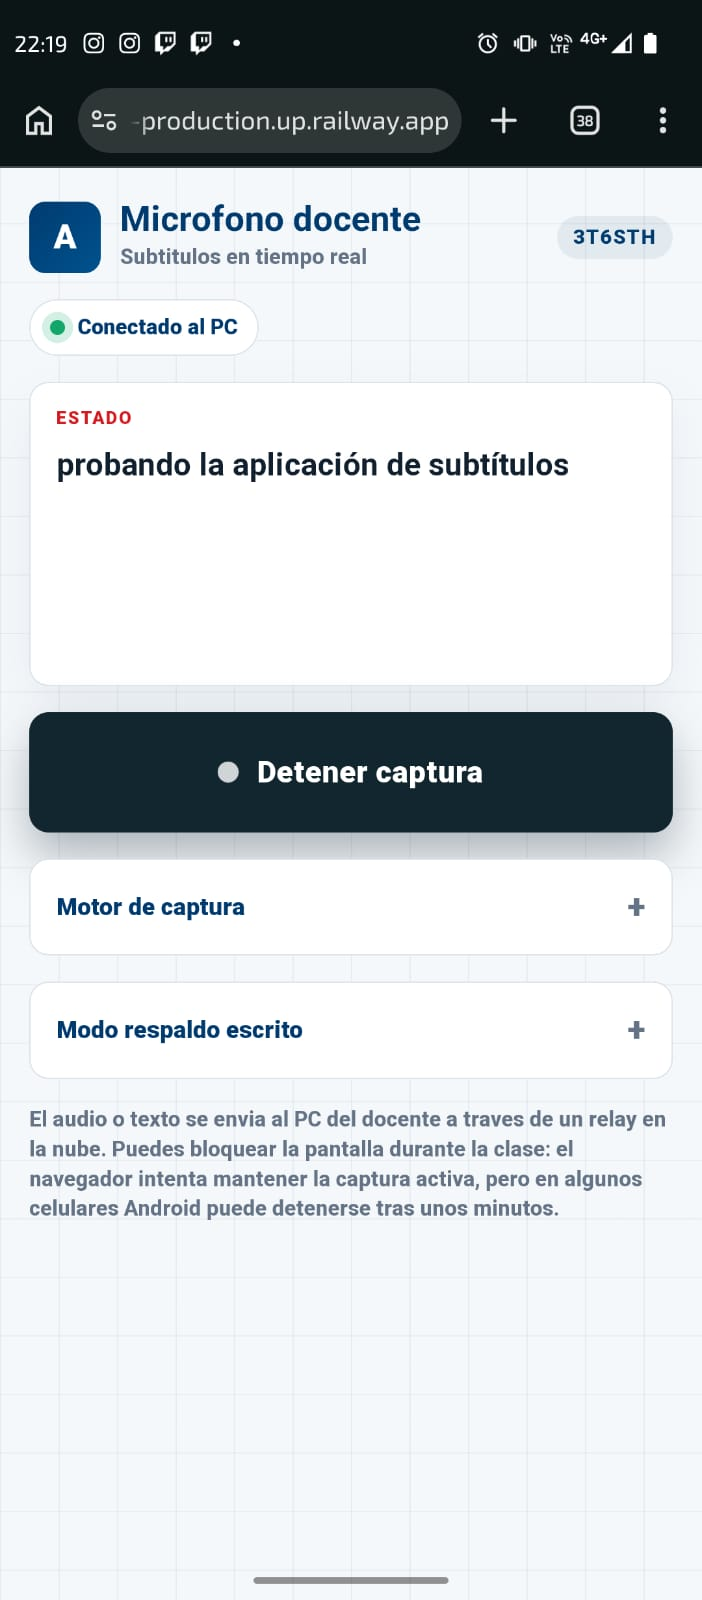
\includegraphics[width=\linewidth]{postulacion-assets/movil-captura-activa.jpeg}
  \imagecaption{\textbf{Captura activa.} El texto reconocido se refleja en el PC como subtítulo de apoyo.}
\end{minipage}
\end{center}

\sectiontitle{Estado actual}

El prototipo funcional ya conecta celular y computador, muestra subtítulos flotantes, permite mover el panel en pantalla y registra transcripciones cuando el docente lo autoriza. La postulación busca validarlo pedagógicamente durante el segundo semestre 2026, levantar evidencia de utilidad con estudiantes y preparar una guía para transferir la experiencia a otros contextos. Como proyección, las transcripciones autorizadas podrán transformarse en materiales de apoyo: resúmenes, glosarios, fichas de repaso o infografías breves.

\sectiontitle{Siguiente paso para la postulación}

\begin{tabularx}{\textwidth}{>{\bfseries}p{4.15cm}X}
Pendiente principal & Definir sección o docente complementario para cumplir el mínimo de 15 estudiantes participantes. \\
Apoyo solicitado & Carta de apoyo institucional para adjuntar en la postulación. \\
Resultado esperado & Piloto medido, ajustes del prototipo y material de replicabilidad para la sede. \\
\end{tabularx}

\end{document}
